% Author: Izaak Neutelings (January 2023)
\documentclass[border=1pt,tikz,dvipsnames]{standalone}
\usepackage{amsmath,amssymb} % for \text
\usepackage{physics} % for \abs
\usepackage{xspace} % for \xspace
\usepackage{bm} % for bold math \bm
\usetikzlibrary{positioning} % for position relative to node
\usetikzlibrary{arrows.meta} % for arrow size
\usetikzlibrary{calc} % for computing coordinates
\tikzset{>=latex} % set default arrow head as latex

% VARIABLES
\newcommand{\pt}    {\ensuremath{p_\text{T}}\xspace}
\newcommand{\ptmiss}{\ensuremath{\pt^\text{miss}}\xspace}
\newcommand{\mvis}  {{\ensuremath{m_\text{vis}}}\xspace}
\newcommand{\GeV}   {{\ensuremath{\,\text{Ge\hspace{-.08em}V}}}\xspace}
\newcommand{\ab}[1]{\textbf{\boldmath{#1}}} % bold text & math

% TIKZ STUFF
\colorlet{myred}{red!80!black}
\colorlet{myblue}{blue!80!black}
\colorlet{mygreen}{green!50!black}
\colorlet{myorange}{orange!80!yellow!90!red!90!black}
\tikzstyle{mycomment}=[inner sep=1pt,scale=0.75,align=left]
\tikzstyle{mybox}=[draw,#1!80!black,fill=#1!95!black!20,inner sep=5pt,outer sep=3pt,
                   thick,rounded corners=3pt,align=center,font=\bfseries]
\tikzstyle{mysmallbox}=[mybox=#1,outer sep=1.5pt]
\tikzstyle{myarrow}=[-{Latex[length=8,width=8]},#1!80!black,thick,line cap=round,line width=3]
\tikzstyle{mysmallarrow}=[-{Latex[length=6,width=6]},#1!80!black,thick,line width=1.6]

% CONNECTOR with straight angles
\def\connect[#1](#2)!#3!(#4){
  \draw[#1] (#2) |- ($(#2)!#3!(#4)$) node[pos=0.5] (#2-#4-1) {}
  -| (#4) node[pos=0.5] (#2-#4-2) {}
}

\begin{document}


% JET CATEGORIES with straight lines
\begin{tikzpicture}[scale=1.0]
  \def\h{-1.6} % vertical space between rows
  \def\w{2.6} % horizontal space between two main branches
  
  \node[mysmallbox=myred] (O) at (0,0) {%
    \ab{$\tau\tau$ preselection}};
  
  % JET CATEGORY: 0j
  \node[mysmallbox=myorange] (0j) at (-\w,\h) {%
    0 jet};
  
  % JET CATEGORY: >=1j
  \node[mysmallbox=mygreen] (1j) at (\w,\h) {%
    \ab{$\geq$1 jet}};
  
  % 0j MVIS BINS
  \path (0j)++(0,\h) node[mysmallbox=myorange] (bin2) {%
    bin 1};
  \node[mysmallbox=myorange,left=5pt of bin2] (bin1) {%
    bin 2};
  \node[mysmallbox=myorange,right=5pt of bin2] (bin3) {%
    bin 3};
  
  % B TAGS
  \path (1j)++(-1,\h) node[mysmallbox=mygreen] (0b) {%
    0 b tag};
  \node[mysmallbox=mygreen,right=6pt of 0b] (1b) {%
    \ab{$\geq$1 b tag}};
  
  % ARROWS
  %\connect[mysmallarrow=myorange](O.-95)!0.3!(0j);
  %\connect[mysmallarrow=mygreen](O.-85)!0.3!(1j);
  \connect[mysmallarrow=myred](O)!0.45!(0j);
  \connect[mysmallarrow=myred](O)!0.45!(1j);
  \connect[mysmallarrow=myorange](0j)!0.45!(bin1);
  \connect[mysmallarrow=myorange](0j)!0.45!(bin2);
  \connect[mysmallarrow=myorange](0j)!0.45!(bin3);
  \connect[mysmallarrow=mygreen](1j)!0.45!(0b);
  \connect[mysmallarrow=mygreen](1j)!0.45!(1b);
  
  % LABELS
  \node[mycomment,right=0pt of O] {%
    $\pt>50\GeV$};
  \node[mycomment,below=-1pt] at (O-0j-1.south) {%
    jet $\pt>50\GeV$};
  \node[mycomment,right=0pt of 1j] {%
    $\mvis>100\GeV$};
  
\end{tikzpicture}


% JET CATEGORIES
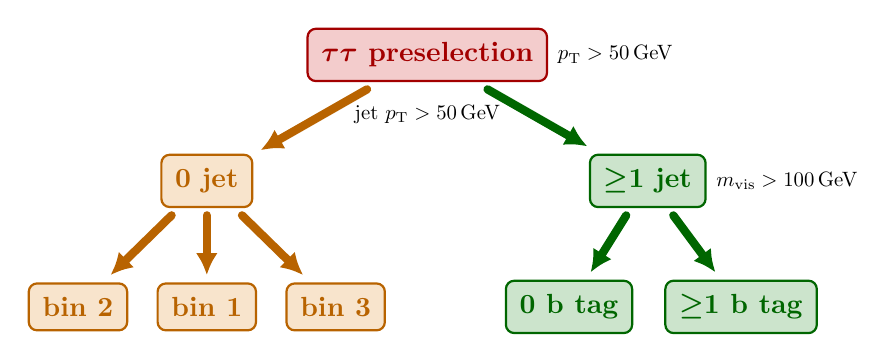
\begin{tikzpicture}[scale=1.0]
  \def\h{-1.6} % vertical space between rows
  \def\w{2.8} % horizontal space between two main branches
  
  \node[mybox=myred] (O) at (0,0) {%
    \ab{$\tau\tau$ preselection}};
  
  % JET CATEGORY: 0j
  \node[mybox=myorange] (0j) at (-\w,\h) {%
    0 jet};
  
  % JET CATEGORY: >=1j
  %\draw[mybox=mygreen] (-0.3,\h) rectangle++ (6.8,3.1*\h);
  \node[mybox=mygreen] (1j) at (\w,\h) {%
    \ab{$\geq$1 jet}};
  
  % 0j MVIS BINS
  \node[mybox=myorange] (bin2) at (-\w,2*\h) {%
    bin 1};
  \node[mybox=myorange,left=5pt of bin2] (bin1) {%
    bin 2};
  \node[mybox=myorange,right=5pt of bin2] (bin3) {%
    bin 3};
  
  % B TAGS
  \node[mybox=mygreen] (0b) at (\w-1,2*\h) {%
    0 b tag};
  \node[mybox=mygreen,right=6pt of 0b] (1b) {%
    \ab{$\geq$1 b tag}};
  
  % ARROWS
  \draw[myarrow=myorange] (O) -- (0j);
  \draw[myarrow=mygreen] (O) -- (1j);
  \draw[myarrow=myorange] (0j) -- (bin1);
  \draw[myarrow=myorange] (0j) -- (bin2);
  \draw[myarrow=myorange] (0j) -- (bin3);
  \draw[myarrow=mygreen] (1j) -- (0b);
  \draw[myarrow=mygreen] (1j) -- (1b);
  
  % LABELS
  \node[mycomment,right=0pt of O] {%
    $\pt>50\GeV$};
  \node[mycomment,below=5pt of O] {%
    jet $\pt>50\GeV$};
  \node[mycomment,right=0pt of 1j] {%
    $\mvis>100\GeV$};
  
\end{tikzpicture}


\end{document}